\documentclass[12pt]{article}

\usepackage{sbc-template}
\usepackage{graphicx,url}
\usepackage[utf8]{inputenc}
\usepackage[brazil]{babel}
\usepackage{booktabs}
\usepackage{amsmath}

\sloppy

\title{Classificação de Moscas em Armadilhas Adesivas com Redes Neurais}

\author{Autor 1\inst{1}, Autor 2\inst{1}, Autor 3\inst{1}, Autor 4\inst{1}}

\address{Instituição de Ensino\\
  Cidade -- Estado -- Brasil
  \email{\{autor1,autor2,autor3,autor4\}@exemplo.com}}

\begin{document}

\maketitle

\begin{abstract}
This work investigates the binary classification of insect crops provided by
Embrapa, distinguishing whitefly samples from other insects collected in yellow
sticky traps. Three approaches were evaluated: a geometric baseline based on
bounding-box attributes, a multilayer perceptron, and a convolutional neural
network. During the methodological revision, a leakage problem was identified
in the crop-level split, because multiple crops originated from the same
original image. The final evaluation was therefore redone with a split by
original image. The results indicate that the dataset is highly separable by
geometry, but also show that the convolutional model provides the best balance
between Average Precision and operational performance for the minority class.
\end{abstract}

\begin{resumo}
Este trabalho investiga a classificação binária de recortes de insetos
fornecidos pela Embrapa, distinguindo amostras de mosca-branca de amostras de
outros insetos presentes em armadilhas adesivas amarelas. Foram avaliadas três
abordagens: um baseline geométrico baseado em atributos do bounding box, um
perceptron multicamadas e uma rede neural convolucional. Durante a revisão
metodológica, foi identificado um problema de vazamento na divisão por
recortes, já que vários recortes provinham da mesma imagem original. A
avaliação final foi então refeita com divisão por imagem de origem. Os
resultados indicam que o conjunto é altamente separável por geometria, mas
também mostram que o modelo convolucional apresenta o melhor equilíbrio entre
Average Precision e desempenho operacional para a classe minoritária.
\end{resumo}

\section{Introdução}

A mosca-branca está entre as pragas de maior impacto na agricultura, tanto pelo
danos diretos às plantas quanto pelo papel de vetor de patógenos. Em cenários
de produção comercial, o monitoramento da infestação é parte importante da
tomada de decisão, pois influencia o controle químico, o manejo integrado de
pragas e a avaliação de risco em diferentes fases do cultivo. No entanto, o
monitoramento manual tende a ser demorado, cansativo e sujeito a variabilidade
humana. Por esse motivo, métodos automáticos de visão computacional e
aprendizado de máquina têm sido considerados uma alternativa promissora para
acelerar e padronizar esse processo \cite{jige2017,barbedo2014}.

O problema estudado neste trabalho foi formulado como uma tarefa de
classificação binária sobre recortes de insetos previamente extraídos de
armadilhas adesivas. O conjunto de dados disponibilizado contém duas classes:
\texttt{WF}, correspondente à mosca-branca, e \texttt{MR}, correspondente aos
demais insetos presentes nas armadilhas. Embora o enunciado da atividade
oriente a exploração de redes neurais convolucionais, a análise foi organizada
de modo a não assumir de antemão que a CNN seria superior em qualquer cenário.
Ao contrário, a proposta foi comparar arquiteturas neurais com um baseline
geométrico simples e, a partir dos resultados, discutir de forma honesta quais
pistas do conjunto de dados estão de fato sendo usadas pelos modelos.

Um ponto central desta versão final do trabalho é a revisão metodológica do
protocolo de avaliação. Em uma primeira formulação, seria natural dividir o
conjunto diretamente por recorte, já que a unidade de classificação é o
recorte individual. Contudo, essa estratégia introduz um problema importante:
muitos recortes diferentes foram produzidos a partir da mesma imagem original da
armadilha. Se alguns desses recortes forem usados no treino e outros no teste,
o modelo será avaliado em exemplos que compartilham contexto visual com
imagens já vistas. Esse fenômeno, conhecido como vazamento entre treino e
teste, pode produzir resultados excessivamente otimistas. A correção desse
problema não enfraquece a escolha da CNN; ao contrário, torna a comparação mais
confiável. Se a CNN permanece forte mesmo em uma avaliação mais rigorosa, então
sua defesa fica tecnicamente mais sólida.

Com isso em mente, os objetivos deste trabalho foram quatro. O primeiro foi
montar e caracterizar o conjunto de dados a partir das pastas \texttt{WF} e
\texttt{MR}. O segundo foi definir um protocolo de divisão sem vazamento,
respeitando a imagem original de origem de cada recorte. O terceiro foi avaliar
três abordagens distintas: um baseline geométrico, um perceptron multicamadas
(MLP) e uma rede neural convolucional (CNN). O quarto foi interpretar os
resultados de forma crítica, distinguindo desempenho real de atalho geométrico
e separando a noção de ranqueamento de probabilidades da noção de decisão final
em um threshold fixo.

\section{Conjunto de Dados e Análise Exploratória}

O conjunto de dados utilizado neste projeto deriva de imagens de armadilhas
adesivas amarelas. As anotações originais foram fornecidas em formato Pascal
VOC e, a partir dos bounding boxes, foram gerados recortes individuais de cada
objeto. A estrutura disponibilizada ao grupo já separava esses recortes em duas
pastas de interesse para a atividade: \texttt{WF}, contendo recortes da
mosca-branca, e \texttt{MR}, contendo recortes de outros insetos.

No total, foram contabilizados 6.350 recortes da classe \texttt{WF} e 1.287
recortes da classe \texttt{MR}. Esse desbalanceamento é relevante porque afeta
o treinamento e a interpretação das métricas. Em uma base assimétrica, um
modelo pode alcançar medidas agregadas aparentemente elevadas mesmo apresentando
comportamento fraco sobre a classe minoritária. Por isso, desde o início da
análise foi considerada a necessidade de observar métricas específicas para
\texttt{MR}.

\begin{figure}[ht]
\centering
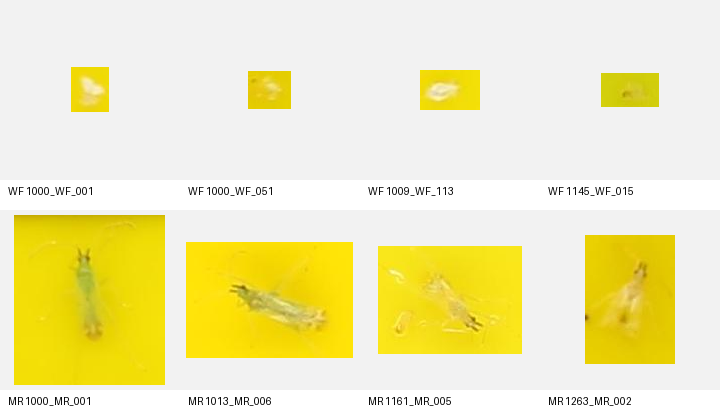
\includegraphics[width=.85\textwidth]{amostras_moscas.png}
\caption{Exemplos de recortes das classes \texttt{WF} e \texttt{MR}. Os
recortes de mosca-branca tendem a ser menores e mais compactos, enquanto os da
classe \texttt{MR} costumam ocupar área maior e apresentar formato mais
alongado.}
\label{fig:amostras}
\end{figure}

Além do desbalanceamento, a inspeção exploratória dos recortes revelou um traço
marcante do conjunto: os objetos da classe \texttt{WF} tendem a ocupar uma área
muito menor do que os da classe \texttt{MR}. Em muitos casos, a mosca-branca
aparece como uma pequena mancha clara sobre o fundo amarelo, enquanto os
insetos da classe \texttt{MR} apresentam corpo mais alongado, maior extensão
espacial e detalhes estruturais mais visíveis. Essa diferença sugere que a
geometria do bounding box, por si só, já pode fornecer informação muito forte
para a tarefa.

Para tornar essa hipótese mensurável, foram calculados quatro atributos
geométricos simples para cada recorte: largura, altura, área e razão de
aspecto. A motivação dessa extração não foi substituir a modelagem visual por
uma solução ad hoc, mas criar um controle experimental. Se esses quatro
atributos já forem suficientes para separar quase completamente as classes,
então qualquer desempenho alto de uma rede neural precisará ser interpretado
com mais cautela. Em outras palavras, o objetivo foi separar o que vem de
aprendizado visual propriamente dito do que já está embutido no tamanho e na
forma global dos recortes.

\begin{figure}[ht]
\centering
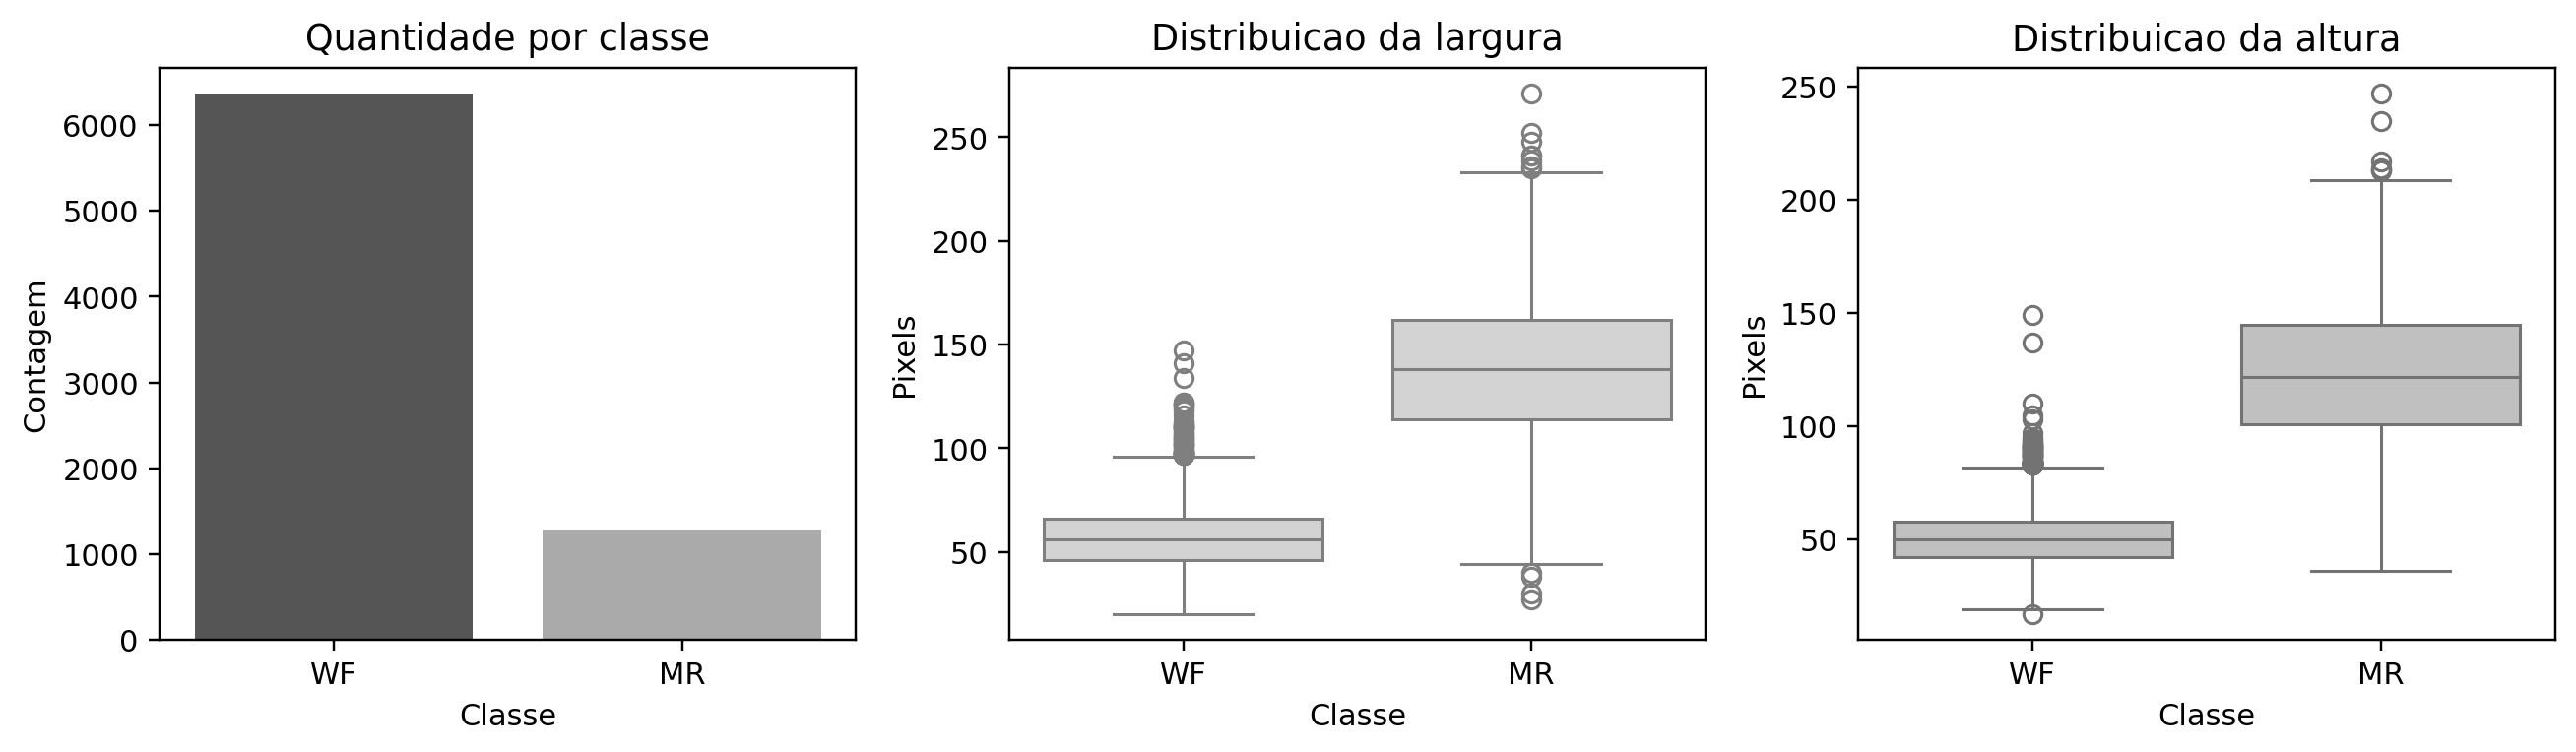
\includegraphics[width=.95\textwidth]{distribuicao_recortes.png}
\caption{Distribuição da quantidade de amostras por classe e das dimensões dos
recortes. A figura evidencia o desbalanceamento do conjunto e a diferença de
escala entre \texttt{WF} e \texttt{MR}.}
\label{fig:distribuicao}
\end{figure}

\section{Correção do Protocolo de Avaliação}

O aspecto metodológico mais importante desta entrega foi a correção do split
entre treino, validação e teste. Em uma divisão ingênua por recorte, diferentes
objetos da mesma imagem original podem cair em partições distintas. Isso gera
vazamento porque o modelo deixa de ser avaliado em exemplos realmente
independentes. Em termos concretos, é possível treinar com alguns recortes da
imagem original \texttt{1000} e depois avaliar com outros recortes extraídos da
mesma armadilha. Ainda que o inseto específico do teste não tenha sido visto,
parte do contexto visual daquele cenário já esteve presente durante o treino.

Esse tipo de sobreposição é particularmente problemático quando os recortes
compartilham fundo, iluminação, textura da armadilha ou distribuição local de
objetos. O risco, nesse caso, não é apenas memorizar o inseto individual, mas
aprender pistas indiretas ligadas à fotografia original. Como consequência, o
teste se torna mais fácil do que deveria e deixa de representar adequadamente a
generalização para novas imagens.

Para eliminar esse problema, a divisão final foi realizada por grupo, usando o
identificador da imagem original como chave. Esse identificador aparece no nome
do arquivo de cada recorte. Por exemplo, \texttt{1000\_WF\_001.jpg} e
\texttt{1000\_MR\_001.jpg} pertencem ao mesmo grupo de origem. O procedimento
adotado foi um \texttt{GroupShuffleSplit} em duas etapas. Primeiro, o conjunto
foi separado em treino+validação e teste. Em seguida, a partição de
treino+validação foi dividida novamente em treino e validação, sempre
preservando os grupos.

Na execução local de referência, a divisão final resultou em 5.569 amostras
distribuídas em 148 grupos para treino, 936 amostras distribuídas em 32 grupos
para validação e 1.132 amostras distribuídas em 32 grupos para teste. A
verificação de interseção entre grupos confirmou ausência de sobreposição entre
as três partições. Isso significa que nenhuma imagem original apareceu em mais
de um conjunto.

Essa mudança metodológica não entra em conflito com a justificativa da CNN.
Pelo contrário. Uma justificativa técnica se fortalece quando permanece válida
sob avaliação mais rigorosa. Se o modelo convolucional ainda apresenta bom
desempenho depois que o teste deixa de compartilhar contexto com o treino,
então sua escolha se apoia menos em artefatos do dataset e mais em sua
adequação real à natureza visual da tarefa.

\section{Modelagem e Pré-processamento}

Três abordagens foram avaliadas. A primeira foi um baseline geométrico
construído com regressão logística sobre os quatro atributos extraídos de cada
recorte. A segunda foi um MLP que recebe a imagem achatada em um vetor
unidimensional. A terceira foi a CNN escolhida como modelo principal.

O baseline geométrico foi importante porque produz uma medida de referência
direta sobre o poder discriminativo do tamanho e da forma global do recorte. O
MLP, por sua vez, permite comparar uma arquitetura neural densa com a CNN sem
qualquer mecanismo explícito de exploração local da imagem. Ao achatar os
pixels em um vetor, o MLP perde a organização espacial da entrada. Isso
significa que relações de vizinhança entre pixels precisam ser reaprendidas de
forma indireta, por meio de uma grande quantidade de parâmetros totalmente
conectados.

A CNN foi escolhida porque imagens possuem organização local. Pixels vizinhos
formam bordas, contornos, manchas claras, alongamentos e pequenas estruturas.
Convoluções foram projetadas justamente para explorar esse tipo de regularidade
local, reaplicando os mesmos filtros ao longo da imagem. Por isso, uma CNN
costuma ser mais adequada do que um MLP quando a entrada é visual.

No pré-processamento, o MLP recebeu imagens redimensionadas para 32x32 pixels.
No caso da CNN, foi adotado um pipeline mais cuidadoso. Antes do resize, cada
recorte foi completado com \textit{padding} até formar uma imagem quadrada.
Essa escolha foi importante porque os recortes possuem proporções muito
diferentes. Um resize direto para 64x64 deformaria artificialmente a geometria
do inseto, o que poderia alterar justamente a pista visual que se deseja
modelar. Após o padding, os recortes foram redimensionados para 64x64,
submetidos a espelhamento horizontal aleatório, pequenas rotações e
normalização dos canais.

Do ponto de vista do treinamento, o conjunto desbalanceado exigiu atenção
especial. Para reduzir a dominância da classe \texttt{WF}, foi utilizado
\texttt{WeightedRandomSampler} nos modelos neurais. Com isso, a classe
minoritária passou a ser apresentada com maior frequência relativa ao modelo
durante o treino, sem necessidade de descartar amostras da classe majoritária.

\section{Treinamento e Métricas}

Os modelos neurais foram treinados com a função de perda
\texttt{BCEWithLogitsLoss} e otimizador Adam. O MLP utilizou taxa de aprendizado
igual a $10^{-3}$, enquanto a CNN foi treinada com taxa de $8 \times 10^{-4}$.
A seleção do melhor ponto foi feita com base no melhor valor de Average
Precision no conjunto de validação.

É importante distinguir as quantidades que aparecem ao longo dos experimentos.
A \textit{loss} é a função numérica otimizada durante o treinamento. Quanto
menor seu valor, melhor o ajuste do modelo aos rótulos observados. Já a
Average Precision, abreviada como AP, resume a qualidade da curva
Precisão-Revocação ao considerar todos os limiares possíveis de decisão
\cite{davis2006}. Em outras palavras, a AP avalia o quão bem o modelo ordena
as amostras da classe positiva ao longo de diferentes thresholds.

Essa distinção é importante porque AP alta não garante, sozinha, comportamento
operacional forte em um threshold específico. Um modelo pode ranquear bem as
amostras e ainda assim apresentar precisão ruim para a classe minoritária
quando se fixa o limiar em 0,5. Por esse motivo, além da AP, também foram
registradas precisão, revocação e acurácia no threshold 0,5, com atenção
especial à classe \texttt{MR}.

\section{Resultados}

Os resultados finais obtidos no teste com split por grupo estão resumidos na
Tabela~\ref{tab:resultados}. O baseline geométrico alcançou AP igual a 0,9994,
o que confirma a hipótese de que largura, altura, área e razão de aspecto já
explicam grande parte da tarefa. O MLP atingiu AP de 0,9963, mas apresentou
precisão de apenas 0,6457 para a classe \texttt{MR} no threshold 0,5. A CNN,
por sua vez, alcançou AP de 0,99999, precisão de 0,9829 para \texttt{MR},
revocação de 1,0000 para \texttt{MR} e acurácia de 0,9974.

\begin{table}[ht]
\centering
\caption{Resultados no conjunto de teste com split por imagem original}
\label{tab:resultados}
\begin{tabular}{lccccc}
\toprule
Modelo & Parâmetros & AP & Prec. MR & Rev. MR & Acurácia \\
\midrule
Geométrico & -- & 0,9994 & 0,9429 & 0,9593 & 0,9850 \\
MLP & 803.201 & 0,9963 & 0,6457 & 0,9535 & 0,9134 \\
CNN & 79.225 & 0,99999 & 0,9829 & 1,0000 & 0,9974 \\
\bottomrule
\end{tabular}
\end{table}

Esses valores exigem interpretação cuidadosa. O número 1,0000 associado à
revocação de \texttt{MR} não significa que a CNN tenha acertado tudo. Esse
valor indica apenas que, naquele conjunto de teste e naquele threshold, todas
as amostras reais de \texttt{MR} foram recuperadas. Isso não implica ausência
de falsos positivos, como mostra a precisão de 0,9829, inferior a 1.

Do ponto de vista comparativo, três conclusões se destacam. Em primeiro lugar,
o dataset é quase totalmente separável por geometria simples. Em segundo lugar,
AP alta, isoladamente, não basta para descrever o comportamento real do modelo.
Em terceiro lugar, a CNN apresentou o melhor equilíbrio entre ranqueamento de
probabilidades e decisão binária final para a classe minoritária.

\section{Discussão}

Os resultados obtidos mostram que a avaliação correta da tarefa exige reconhecer
dois fatos simultâneos. O primeiro é que o dataset contém um atalho geométrico
muito forte. O baseline logístico baseado apenas em atributos do bounding box
foi suficiente para produzir desempenho extremamente alto. Isso significa que
uma parte importante do problema pode ser resolvida sem necessidade de
aprendizado visual profundo.

O segundo fato é que, mesmo assim, a CNN continua sendo a melhor escolha final
entre os modelos neurais avaliados. Essa afirmação não depende de uma
justificativa vaga do tipo ``CNN é melhor porque é imagem'', nem da existência
de vazamento entre treino e teste. Ela se apoia em um protocolo corrigido, em
que o teste é realmente independente da imagem original usada no treino, e em
um conjunto de métricas que vai além da AP isolada.

Nesse cenário mais rigoroso, a CNN se mostrou superior ao MLP em dois sentidos.
O primeiro é estrutural: convoluções exploram relações locais entre pixels
vizinhos e, portanto, modelam melhor contorno, compactação e alongamento do
inseto. O segundo é empírico: a CNN manteve AP muito alta e apresentou
comportamento operacional claramente melhor para \texttt{MR}. O MLP, por sua
vez, ainda que competitivo em AP, produziu precisão bem inferior para a classe
minoritária quando o limiar foi fixado em 0,5.

Essa diferença também ajuda a interpretar por que remover o vazamento não
contradiz a escolha da CNN. Se a justificativa da CNN dependesse do vazamento,
ela desapareceria assim que o protocolo fosse corrigido. Mas o que se observou
foi o oposto: em avaliação mais rigorosa, a CNN permaneceu forte e ainda se
mostrou superior ao MLP em termos operacionais. Portanto, a revisão
metodológica não enfraquece o argumento; ela o fortalece.

\section{Conclusão}

O trabalho foi concluído com um protocolo experimental mais sólido do que o
planejado inicialmente. A montagem dos dados foi feita a partir das pastas
\texttt{WF} e \texttt{MR}, o split foi corrigido para respeitar a imagem
original de origem de cada recorte, foram treinados modelos neurais e a
avaliação principal foi conduzida por meio de Precisão-Revocação e Average
Precision.

Os resultados mostram que o problema é altamente separável, que a geometria do
recorte é uma pista muito forte e que essa característica precisa ser assumida
explicitamente na interpretação do desempenho. Mesmo com essa limitação, a CNN
permanece como a melhor escolha final entre os modelos neurais avaliados, por
combinar adequação conceitual à natureza visual da entrada com melhor
desempenho empírico sob avaliação sem vazamento.

\begin{thebibliography}{99}

\bibitem{bar2019}
BAR, L. et al. Downregulation of dystrophin expression in pupae of the
whitefly \textit{Bemisia tabaci} inhibits the emergence of adults.
\textit{Insect Molecular Biology}, 2019.

\bibitem{jige2017}
JIGE, M. N.; RATNAPARKHE, V. R. Population estimation of whitefly for cotton
plant using image processing approach. In: \textit{2017 2nd IEEE International
Conference on Recent Trends in Electronics, Information \& Communication
Technology}. 2017.

\bibitem{barbedo2014}
BARBEDO, J. G. A. Using digital image processing for counting whiteflies on
soybean leaves. \textit{Journal of Asia-Pacific Entomology}, v. 17, n. 4,
p. 685--694, 2014.

\bibitem{davis2006}
DAVIS, J.; GOADRICH, M. The relationship between Precision-Recall and ROC
curves. In: \textit{Proceedings of the 23rd International Conference on Machine
Learning}. 2006. p. 233--240.

\end{thebibliography}

\end{document}
